\section{Introduction and literature review}\label{S01}

Balancing is an important issue related to the design of mechanical systems in general,
and also parallel mechanisms, in particular. In fact, the performance of parallel mechanisms
associated to specific applications depends on the choice of the balancing method, namely, 
either static or dynamic, either passive or active, whether it is valid for a given trajectory
or even for any motion.

% definition of Static balancing, purpose
In a statically balanced mechanism, the potential energy is invariant. Hence,
the actuator torques/forces are null at any configuration [6].
% definition of Dynamic balancing, purpose
On the other hand, in a dynamically balanced mechanism, the shaking forces and
shaking moments at its frame are reduced or even eliminated. As a consequence, 
the mechanism components are less susceptible to vibration, wear and fatigue [4],
improving its life.

% passive and active balancing
Passive balancing means that the original mechanism
architecture is modified by using some techniques.
The most common techniques are
the addition of counterweights
~\cite{1wijk,2arakelian,3seo,4wu,6wang,7wang,12russo,15coelho,16moradi}, 
the use of counter-rotating inertias~\cite{2arakelian,4wu,15coelho,16moradi} 
and the redistribution of masses~\cite{8alici,9alici}.
Alternatively, other works propose the addition of extra
links~\cite{5gosselin,12russo,13agrawal}.
However, for high speed manipulators, these techniques might cause the increase of the actuator
torques and the size of links and joints.
Hence, in order to avoid such undesirable effects, some 
authors~\cite{6wang,7wang,8alici,9alici,10dehkordi,13agrawal} recommend the use of
 elastic springs attached to the mechanism.

For the active balancing~\cite{2arakelian,3seo,11wang,14briot,15coelho,16moradi}, 
more complex modifications are needed to implement it. 
For instance, the counterweights position in the moving links might be altered
according to the end-effector load or the given trajectory. Hence, 
additional actuators/sensors and control are usually employed to reach satisfactory performance levels. Arakelian and Smith~\cite{2arakelian} employ a computer control of the motion of a inertia flywheel connected to the mechanism.

Moreover, Coelho et al.~\cite{15coelho} and Moradi et al.~\cite{16moradi} use the adaptive balancing to achieve the 
decoupling of dynamic equations for open-loop kinematic chain mechanisms. 
Consequently, this action simplifies the control of manipulators due to the fact that the 
actuators can be controlled independently. 

% esclarecer a contribuição
The main contribution of this work is to highlight the importance of the dynamic modelling 
process (see Figure~\ref{F01-101}) in order to achieve the compensation conditions associated to the chosen 
balancing technique. Due to the fact that parallel mechanisms have highly complex structures,
the use of dynamic formalisms that employ redundant generalized coordinates,
in association with the successive coupling of additional balancing elements 
to the original system model, can bring remarkable benefits.
Additionally, this book chapter also discusses the impact of
the dynamic model, developed in accordance with the methodology shown here, for the 
control strategy of parallel mechanisms.

% seções
This chapter is organized as follows. Section 2 treats of the theoretical background for the dynamic modelling and control, the adaptive balancing techniques are described in section 3, section 4 shows a case study for the planar 5-bar mechanism with revolute joints.  Finally, the conclusions are drawn in section 5.


% shaking force and shaking to keep base vibrations low [1]
% reduction of the variable dynamic loads on
%     the frame and, as a result, a reduction of vibrations [2]
%   However, similar to other robotic
%   devices, they exert forces and moments on their base while
%   moving, causing fatigue, vibration, noise, and disturbances in
%     the supporting structure of the mechanism [4]
% reactionless or dynamically balanced
% if the reaction forces (excluding gravity) and reaction moments—
% or shaking forces and shaking moments—at its base are
% identically equal to zero at all times and for any motion of the mechanism. [4]
% 
% static balancing is defined as the set of conditions under which the weight of the links of the mechanism does not
% produce any torque (or force) at the actuators under static conditions, for any con®guration of
%  the manipulator or mechanism. This condition is also referred to as gravity compensation. [6]
%  unbalanced forces on the base will lead to vibrations, wear and other undesirable side effects.[7]
% gravity compensation condition, the total potential
% energy of the system should remain constant for all of the
% manipulator’s configurations [10]
% constant total potential energy of the
% manipulator for all of its configurations. This follows that the
% manipulator is in equilibrium with zero actuator force, and
% less powerful and smaller actuators can be employed to move it. [8]
% the inertia-induced force (shaking force) and moment (shaking moment) transmitted to the mechanism
% frame. If their magnitudes and directions change throughout the operation of the mechanism, the mechanism
% will vibrate undesirably, and consequently, its dynamic performance will be unsatisfactory. [9]
% a technique that brings some modifications to the original kinematic chain
% of unbalanced mechanisms in such a way to obtain static balancing and complete decoupling of
% dynamic equations, thus eliminating Coriolis, centripetal, gravitational and cross inertia terms,
% even when payload changes. [14]

%
% and the actuator torques. 


% definition of passive and active balancing

% balancing techniques

 

% analytical approach numerical approach

% valid for any motion for given motion

% Simulation
% Experimental tests

\begin{figure}[H]
	\centering
	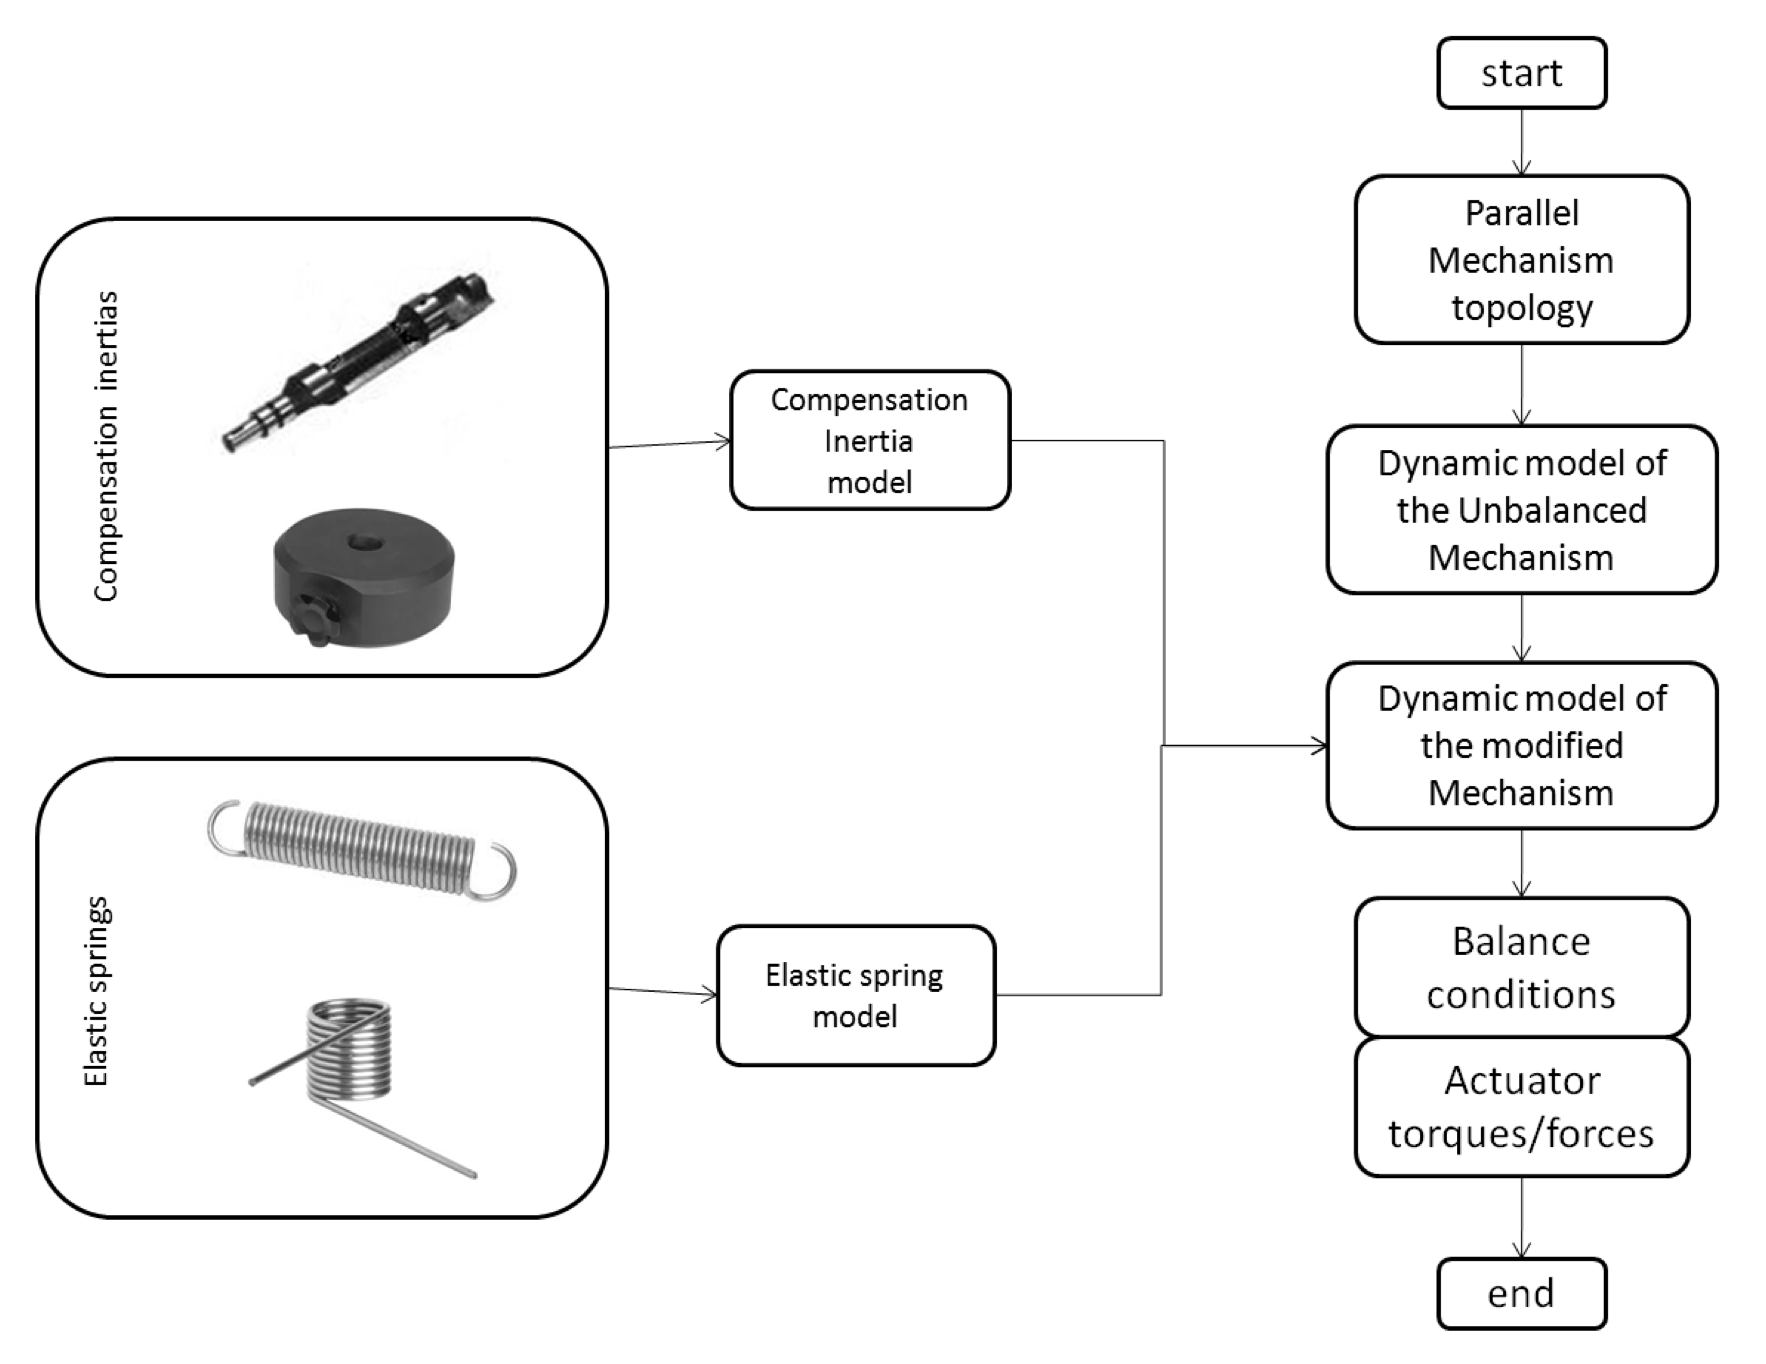
\includegraphics[scale=0.4]{model-1.png}
	\caption{Dynamic modelling process}
	\label{F01-101}
\end{figure}
